\documentclass[aspectratio=169]{beamer}
\usetheme{default}
\usecolortheme{default}
\setbeamertemplate{navigation symbols}{}
\setbeamertemplate{footline}{}
\setbeamercolor{background canvas}{bg=white}
\setbeamercolor{title}{fg=black}
\setbeamercolor{frametitle}{fg=black,bg=white}
\setbeamerfont{frametitle}{series=\bfseries,size=\Large}
\setbeamercolor{block title}{fg=black,bg=white}
\setbeamercolor{normal text}{fg=black}
\setbeamercolor{itemize item}{fg=blue!55!black}
\setbeamercolor{itemize subitem}{fg=blue!55!black}

\usepackage{graphicx}
\usepackage{xcolor}
\usepackage{array}

\definecolor{ink}{HTML}{222733}
\definecolor{muted}{HTML}{5A6373}
\definecolor{accent}{HTML}{2E5FA3}

\newcommand{\kicker}[1]{{\footnotesize\bfseries\color{accent} #1}\\[2pt]}

\begin{document}

% ---------------- Slide 1 ----------------
\begin{frame}[t]
\kicker{EXPLORATORY FOLLOW-UP \textperiodcentered\ NO NEW DATA PULLED}
\frametitle{Does spatial resolution explain the MERRA-2 vs.\ MODSCAG disagreement?}

\begin{columns}[t]
\begin{column}{0.56\textwidth}
\tiny
\begin{itemize}
  \setlength{\itemsep}{2pt}
  \item[] \textbf{Question:} how much of the pooled bias reflects MERRA's coarse $0.625^\circ\!\times\!0.5^\circ$ grid vs.\ some other cause?
  \item[] \textbf{Constraint:} reuse existing outputs only --- no reprocessing/redownload, no change to the aggregation rule (MODIS up to MERRA; never MERRA down).
  \item[] \textbf{Terrain heterogeneity proxy:} bin the checked-in USGS 3DEP DEM ($800\times600$ px) into the 72 MERRA cells; within-cell elevation std.\ dev.\ --- steep, heterogeneous cells are worst represented by a coarse grid.
  \item[] \textbf{Bias signal:} recombine already-computed monthly sufficient stats (\texttt{pixel\_stats.csv} climatology-month rows) per cell into pooled WY2010--2023 bias/NMB, same 5\% low-snow mask as the public figure.
  \item[] \textbf{Two comparisons:} (1) terrain heterogeneity vs.\ spatial bias; (2) spatial vs.\ temporal bias variance.
\end{itemize}
\end{column}

\begin{column}{0.42\textwidth}
\footnotesize
\textbf{Inputs (all pre-existing)}
\vspace{2pt}

\begin{tabular}{@{}p{\linewidth}@{}}
\color{accent}\ttfamily\tiny tests/fixtures/domain\_dem\_3dep.tif \\
\color{muted}\scriptsize real 3DEP DEM, checked in \\[2pt]
\color{accent}\ttfamily\tiny results/water\_year\_2010\_2023\_pixel\_stats.csv \\
\color{muted}\scriptsize per-cell climatology sufficient stats \\[2pt]
\color{accent}\ttfamily\tiny results/water\_year\_2010\_2023\_overall\_stats.csv \\
\color{muted}\scriptsize per-year domain sufficient stats \\
\end{tabular}

\vspace{4pt}
\textbf{\footnotesize New, exploratory-only artifact:}

{\tiny\color{accent}\ttfamily scripts/resolution\_attribution.py $\rightarrow$ results/derived\_resolution\_attribution.\{csv,png\}}
\end{column}
\end{columns}

\vfill
{\tiny\color{muted} Not part of the scientific-contract pipeline or public product; error sign, masks, and grid rules unchanged from README.md.}
\end{frame}

% ---------------- Slide 2 ----------------
\begin{frame}[t]
\kicker{FINDINGS}
\frametitle{Result: bias pattern is mostly not explained by terrain heterogeneity}

\begin{center}
\vspace{-4pt}
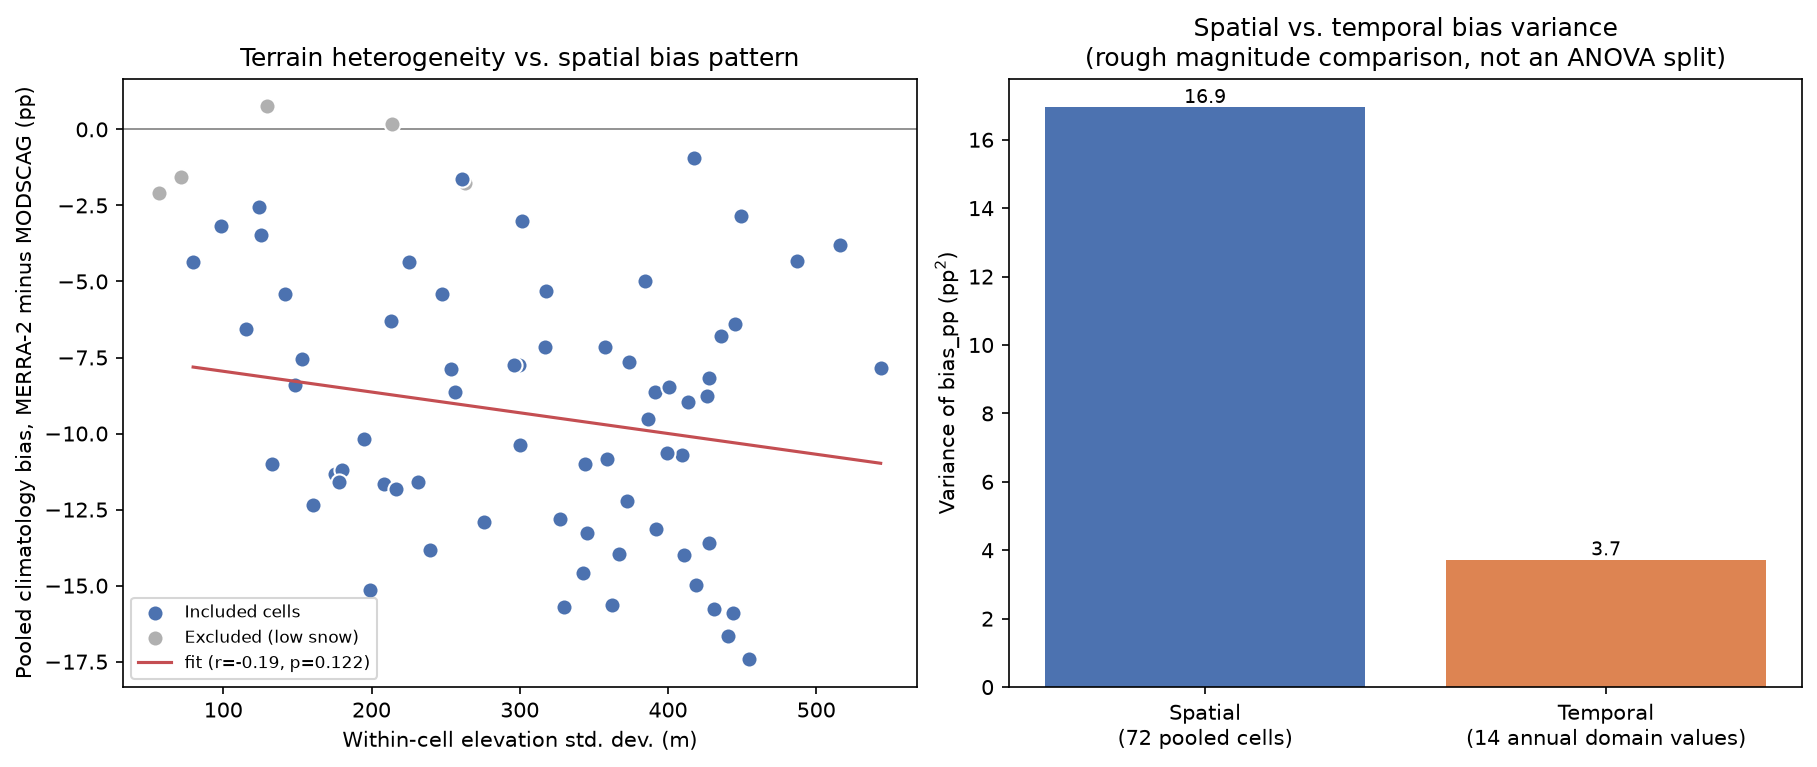
\includegraphics[width=0.5\linewidth]{derived_resolution_attribution.png}
\end{center}

\vspace{-6pt}
\scriptsize
\begin{itemize}
  \setlength{\itemsep}{1pt}
  \item[] \textbf{Correlation:} $r = -0.19$ ($p = 0.12$, $R^2 \approx 0.04$) across 67 of 72 cells (5 masked for low snow) --- essentially no relationship, and the weak trend runs opposite to a resolution-mismatch story.
  \item[] \textbf{Variance split:} spatial variance across cells ($\approx$16.9~pp$^2$) is $\sim$4.5$\times$ the interannual variance at the domain level ($\approx$3.7~pp$^2$) --- the disagreement is mostly a stable spatial pattern, not year-to-year.
  \item[] \textbf{Interpretation:} spatial pattern doesn't track terrain heterogeneity, so resolution/aggregation mismatch looks like a minor contributor. Next: land cover, radiation/snow-physics differences, or a location-dependent MERRA bias unrelated to subgrid relief.
\end{itemize}

\vfill
{\tiny\color{muted} Correlational, not a controlled regridding experiment --- MERRA is never resampled to MODIS resolution in this repository. See \texttt{results/derived\_resolution\_attribution.csv} for full per-cell values.}
\end{frame}

% ---------------- Slide 3 ----------------
\begin{frame}[t]
\kicker{FOLLOW-UP · DOES SNOW AMOUNT EXPLAIN IT INSTEAD?}
\frametitle{\normalsize Bias tracks how much snow a cell has --- but that doesn't isolate resolution}

\begin{columns}[t]
\begin{column}{0.46\textwidth}
\vspace{-2pt}
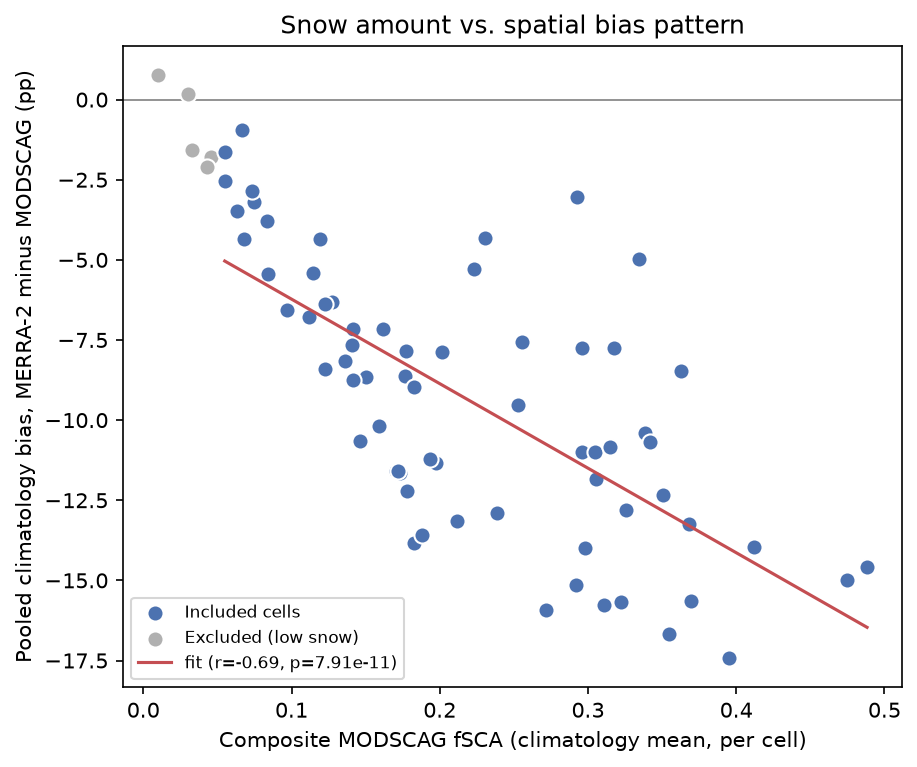
\includegraphics[width=\linewidth]{derived_mixed_pixel_attribution.png}
\end{column}

\begin{column}{0.52\textwidth}
\tiny
\begin{itemize}
  \setlength{\itemsep}{1pt}
  \item[] \textbf{Motivating idea:} finer MODSCAG pixels can resolve a coarse MERRA cell that is partly snow, partly bare; MERRA represents it with one value. Disagreement should be worst in \emph{mixed-state} cells, proxied by fSCA$\times(1-$fSCA$)$, peaking at fSCA$=0.5$.
  \item[] \textbf{What the data show:} every included cell has composite fSCA $< 0.5$ (0.05--0.49) --- on this side of 0.5, fSCA$\times(1-$fSCA$)$ is monotonic in fSCA, so it can't be told apart from raw snow amount here. Raw fSCA vs.\ bias: $r=-0.69$ ($R^2\approx0.48$); mixed-state proxy: $r=-0.72$ ($R^2\approx0.52$) --- nearly the same.
  \item[] \textbf{Honest read:} more snow $\Rightarrow$ more negative bias is real and strong, but can't separate a resolution/mixed-pixel mechanism from other snow-amount-scaling effects (e.g.\ a MERRA depletion-curve or physics bias unrelated to pixel size).
\end{itemize}
\end{column}
\end{columns}

\vfill
{\tiny\color{muted} A direct mixed-pixel test needs within-cell fine-pixel variance, not just the mean --- not recoverable from saved sufficient statistics without reprocessing daily granules.}
\end{frame}

\end{document}
